\documentclass[10pt,a4paper]{scrartcl}
\usepackage[utf8]{inputenc}
\usepackage{amsmath}
\usepackage{amsfonts}
\usepackage{amssymb}
\usepackage{graphicx}

\usepackage[bottom = 1in, left = 0.5in, right = 0.5in, top = 1in]{geometry}

\usepackage[english]{babel}
\usepackage[autostyle]{csquotes}
\usepackage{mathptmx}

\usepackage[labelfont=bf]{caption}

\usepackage[default, scale=0.95]{opensans}

\usepackage[T1]{fontenc}

\usepackage{fixltx2e}

\title{My neat title here}
\subtitle{Figures}
\date{}

\begin{document}
\maketitle

\begin{figure}[h]
	\centering
	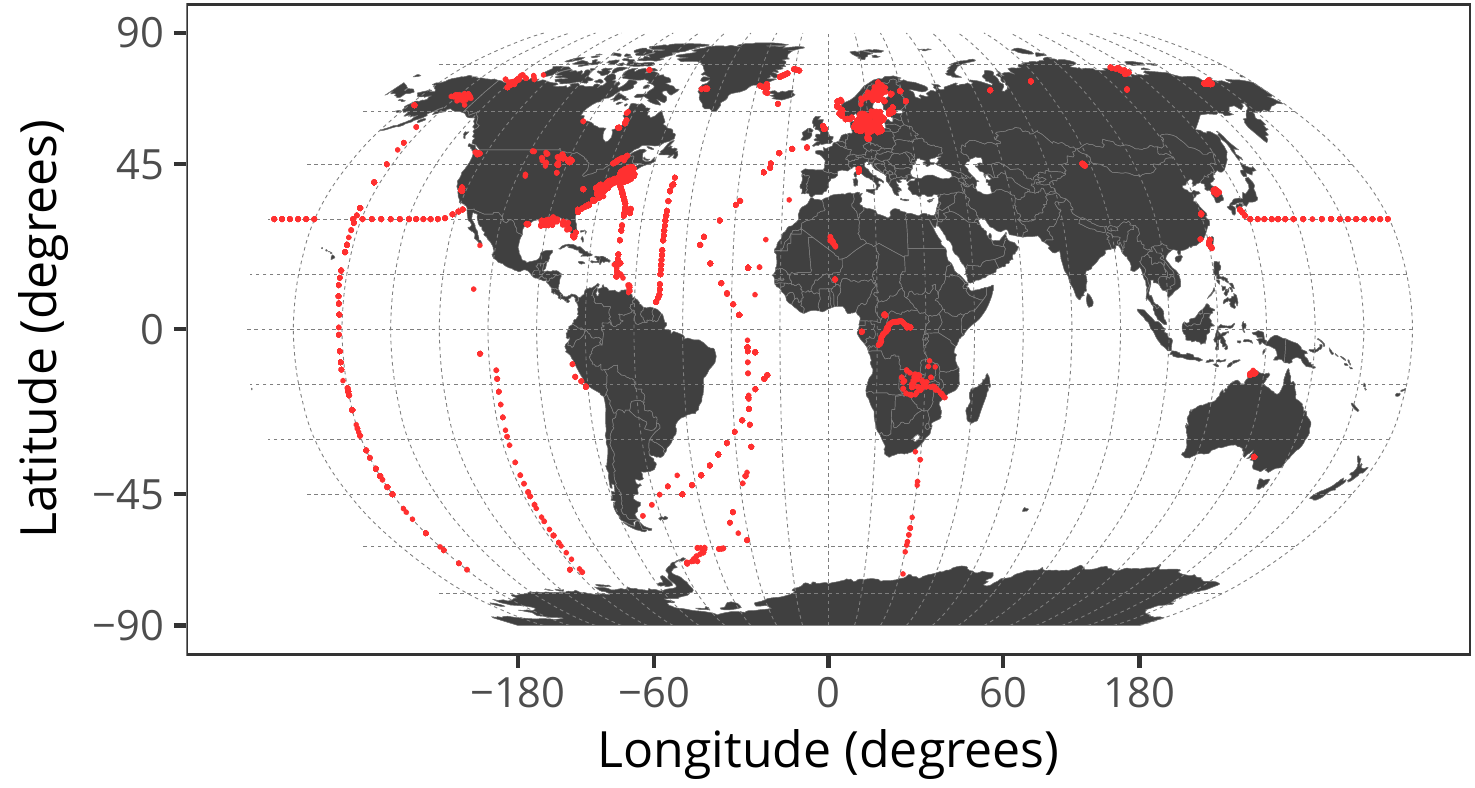
\includegraphics[scale = 1]{../../graphs/fig1}
	\caption{World map showing the spatial distribution of the observations extracted from the literature ($n = xxx$).}
\end{figure}

\clearpage
\newpage

\begin{figure}[h]
	\centering
	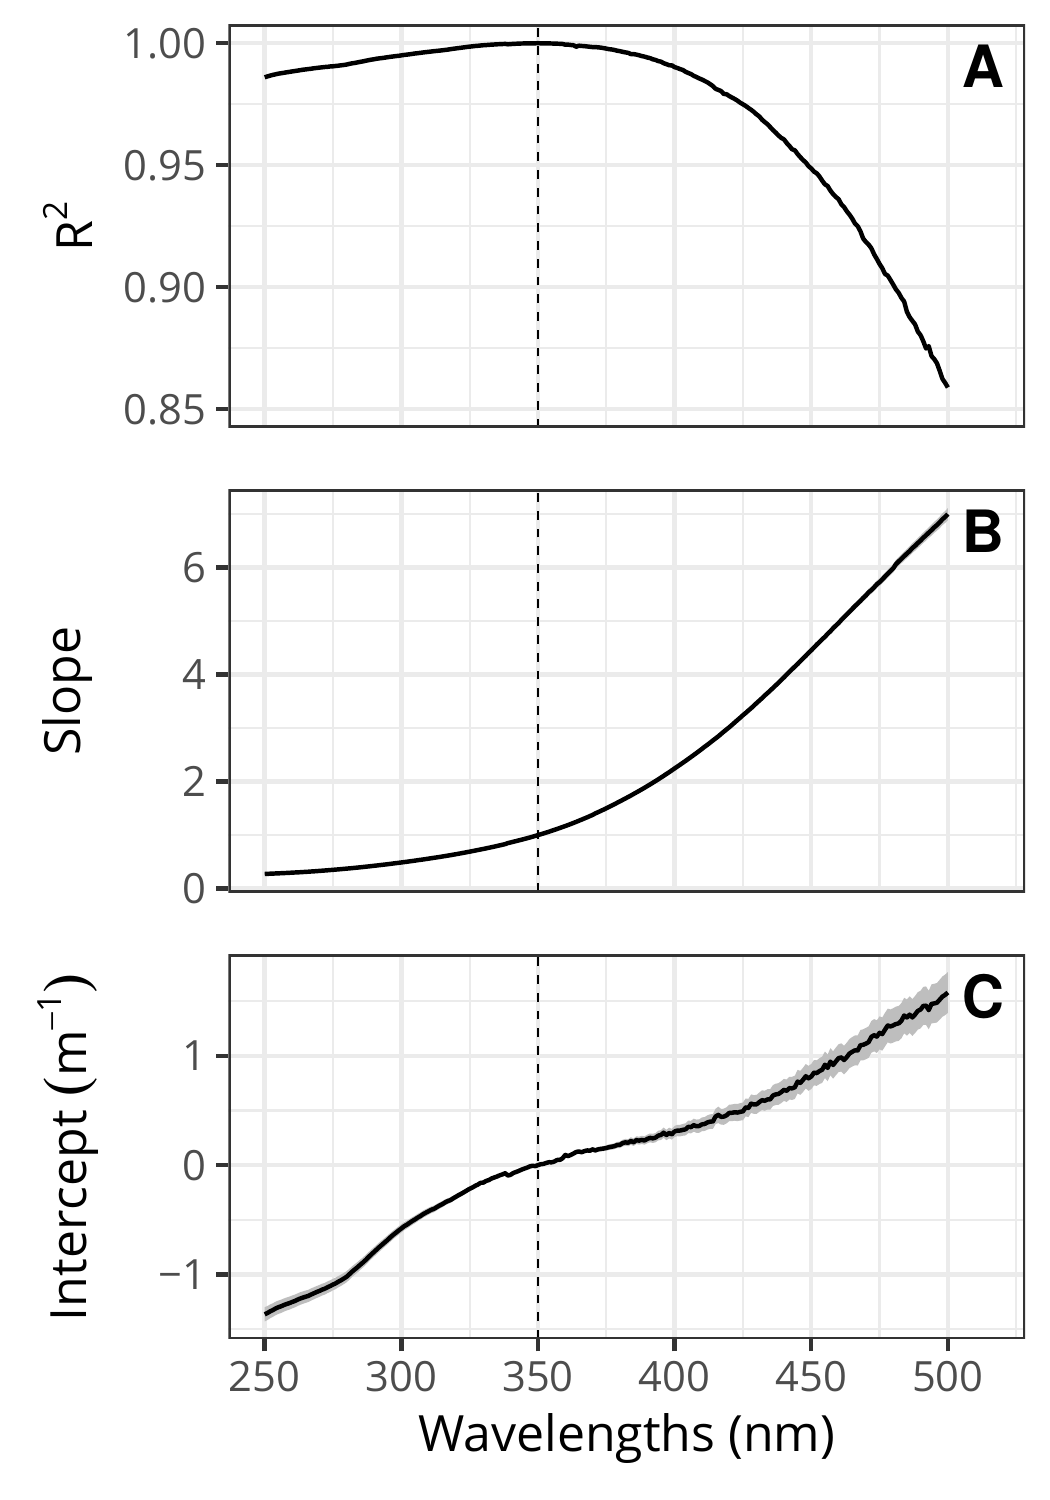
\includegraphics[scale = 1]{../../graphs/fig2}
	\caption{Results of the linear regressions between a\textsubscript{CDOM}(350) and a\textsubscript{CDOM}($\lambda$). (\textbf{A}) Determination coefficients ($R^2$), (\textbf{B}) slopes and (\textbf{C}) intercepts of the linear regressions. Shaded areas (only visible in panel C) show the 95\% confidence interval of the estimated parameters. Panels contain the results of 251 linear models, each based on 2387 data points. Note that at $\lambda = 350$ nm (vertical dashed line), $R^2 = 1$, slope = 1 and intercept = 0.}
\end{figure}

\clearpage
\newpage

\begin{figure}[h]
	\centering
	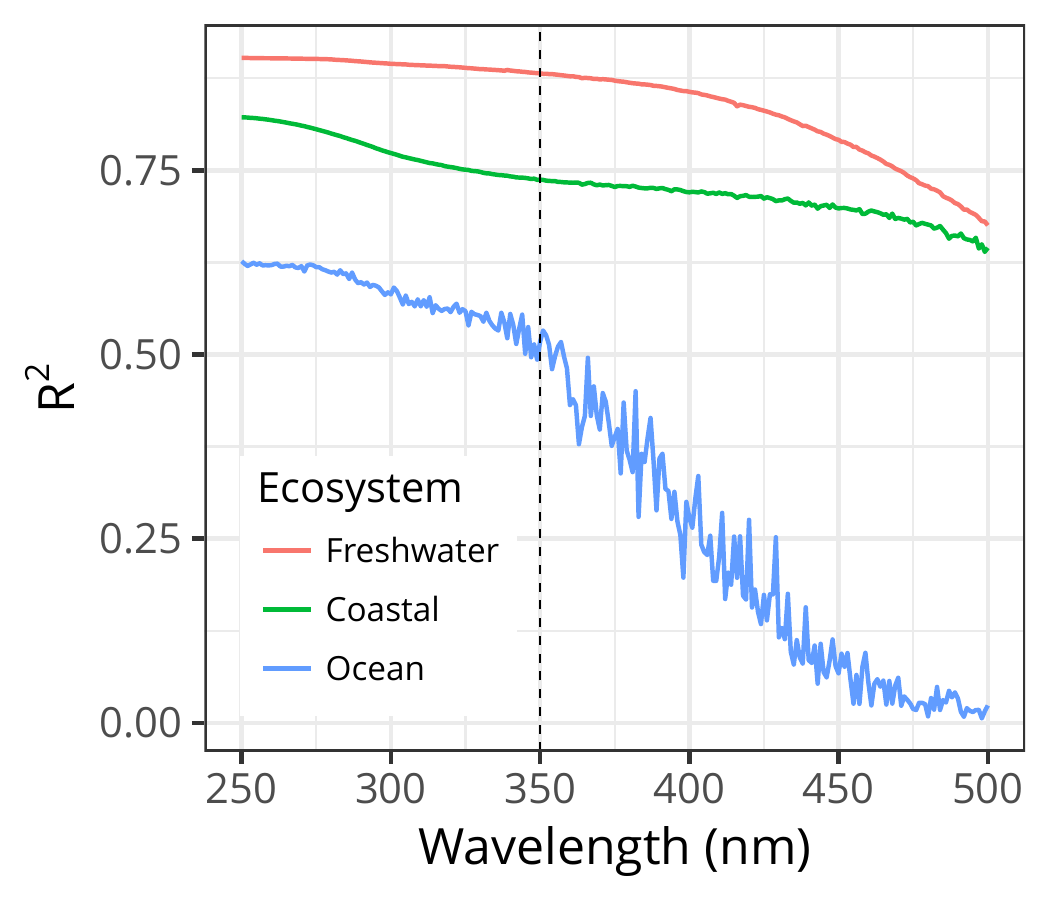
\includegraphics[scale = 0.75]{../../graphs/fig3}
	\caption{Boxplots showing the distribution of (\textbf{A}) absorption coefficients at 350 nm ($a_{CDOM}(350)$), (\textbf{B}) dissolved organic carbon (DOC) and (\textbf{C}) the specific ultra-violet absorbance at 350 nm (SUVA\textsubscript{350}). Y-axis are log-transformed given the wide ranges spanned by the data.}
\end{figure}

\clearpage
\newpage

\begin{figure}[h]
	\centering
	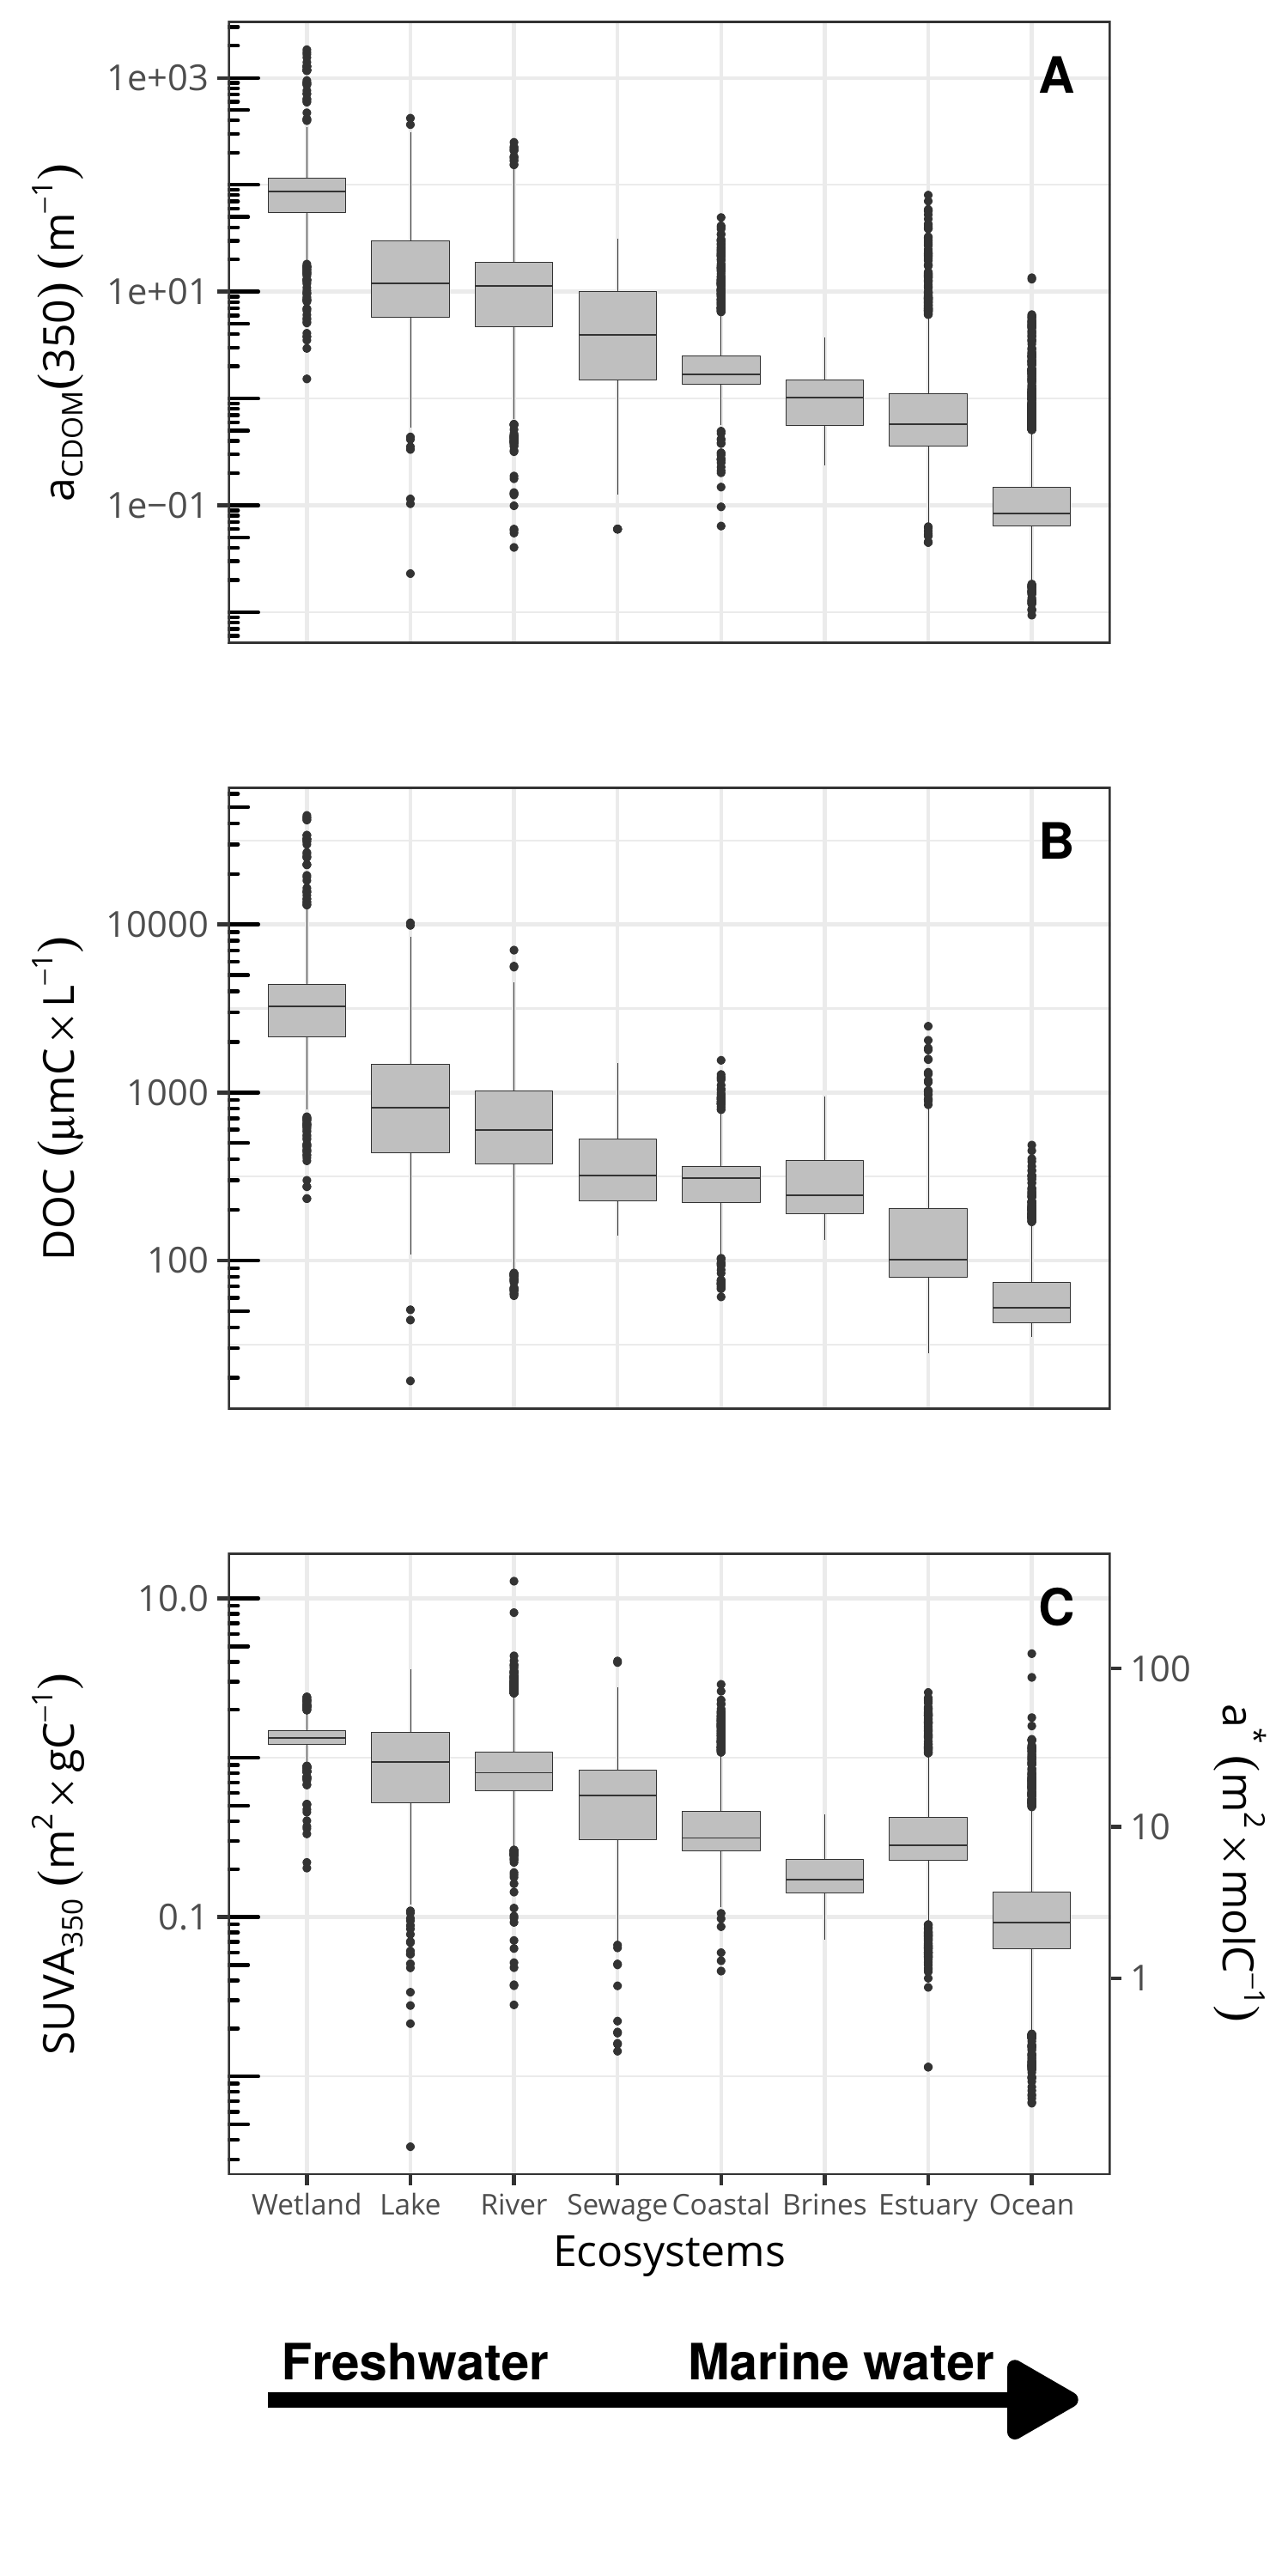
\includegraphics[scale = 1]{../../graphs/fig4}
	\caption{(\textbf{A}) Global relationship between absorption at 350 nm a\textsubscript{CDOM}(350) and dissolved organic carbon. The blue line is the fitted values of a linear model $y~=~log(x), R^2~=~0.93, p~<~0.00001, n~=~11562$. (\textbf{B}) Barplot showing the determination coefficient ($R^2$) of the linear relationships between a\textsubscript{CDOM}(350) and DOC by ecosystems. The dashed horizontal line represents the average of $R^2$.}
\end{figure}

\clearpage
\newpage

\begin{figure}[h]
	\centering
	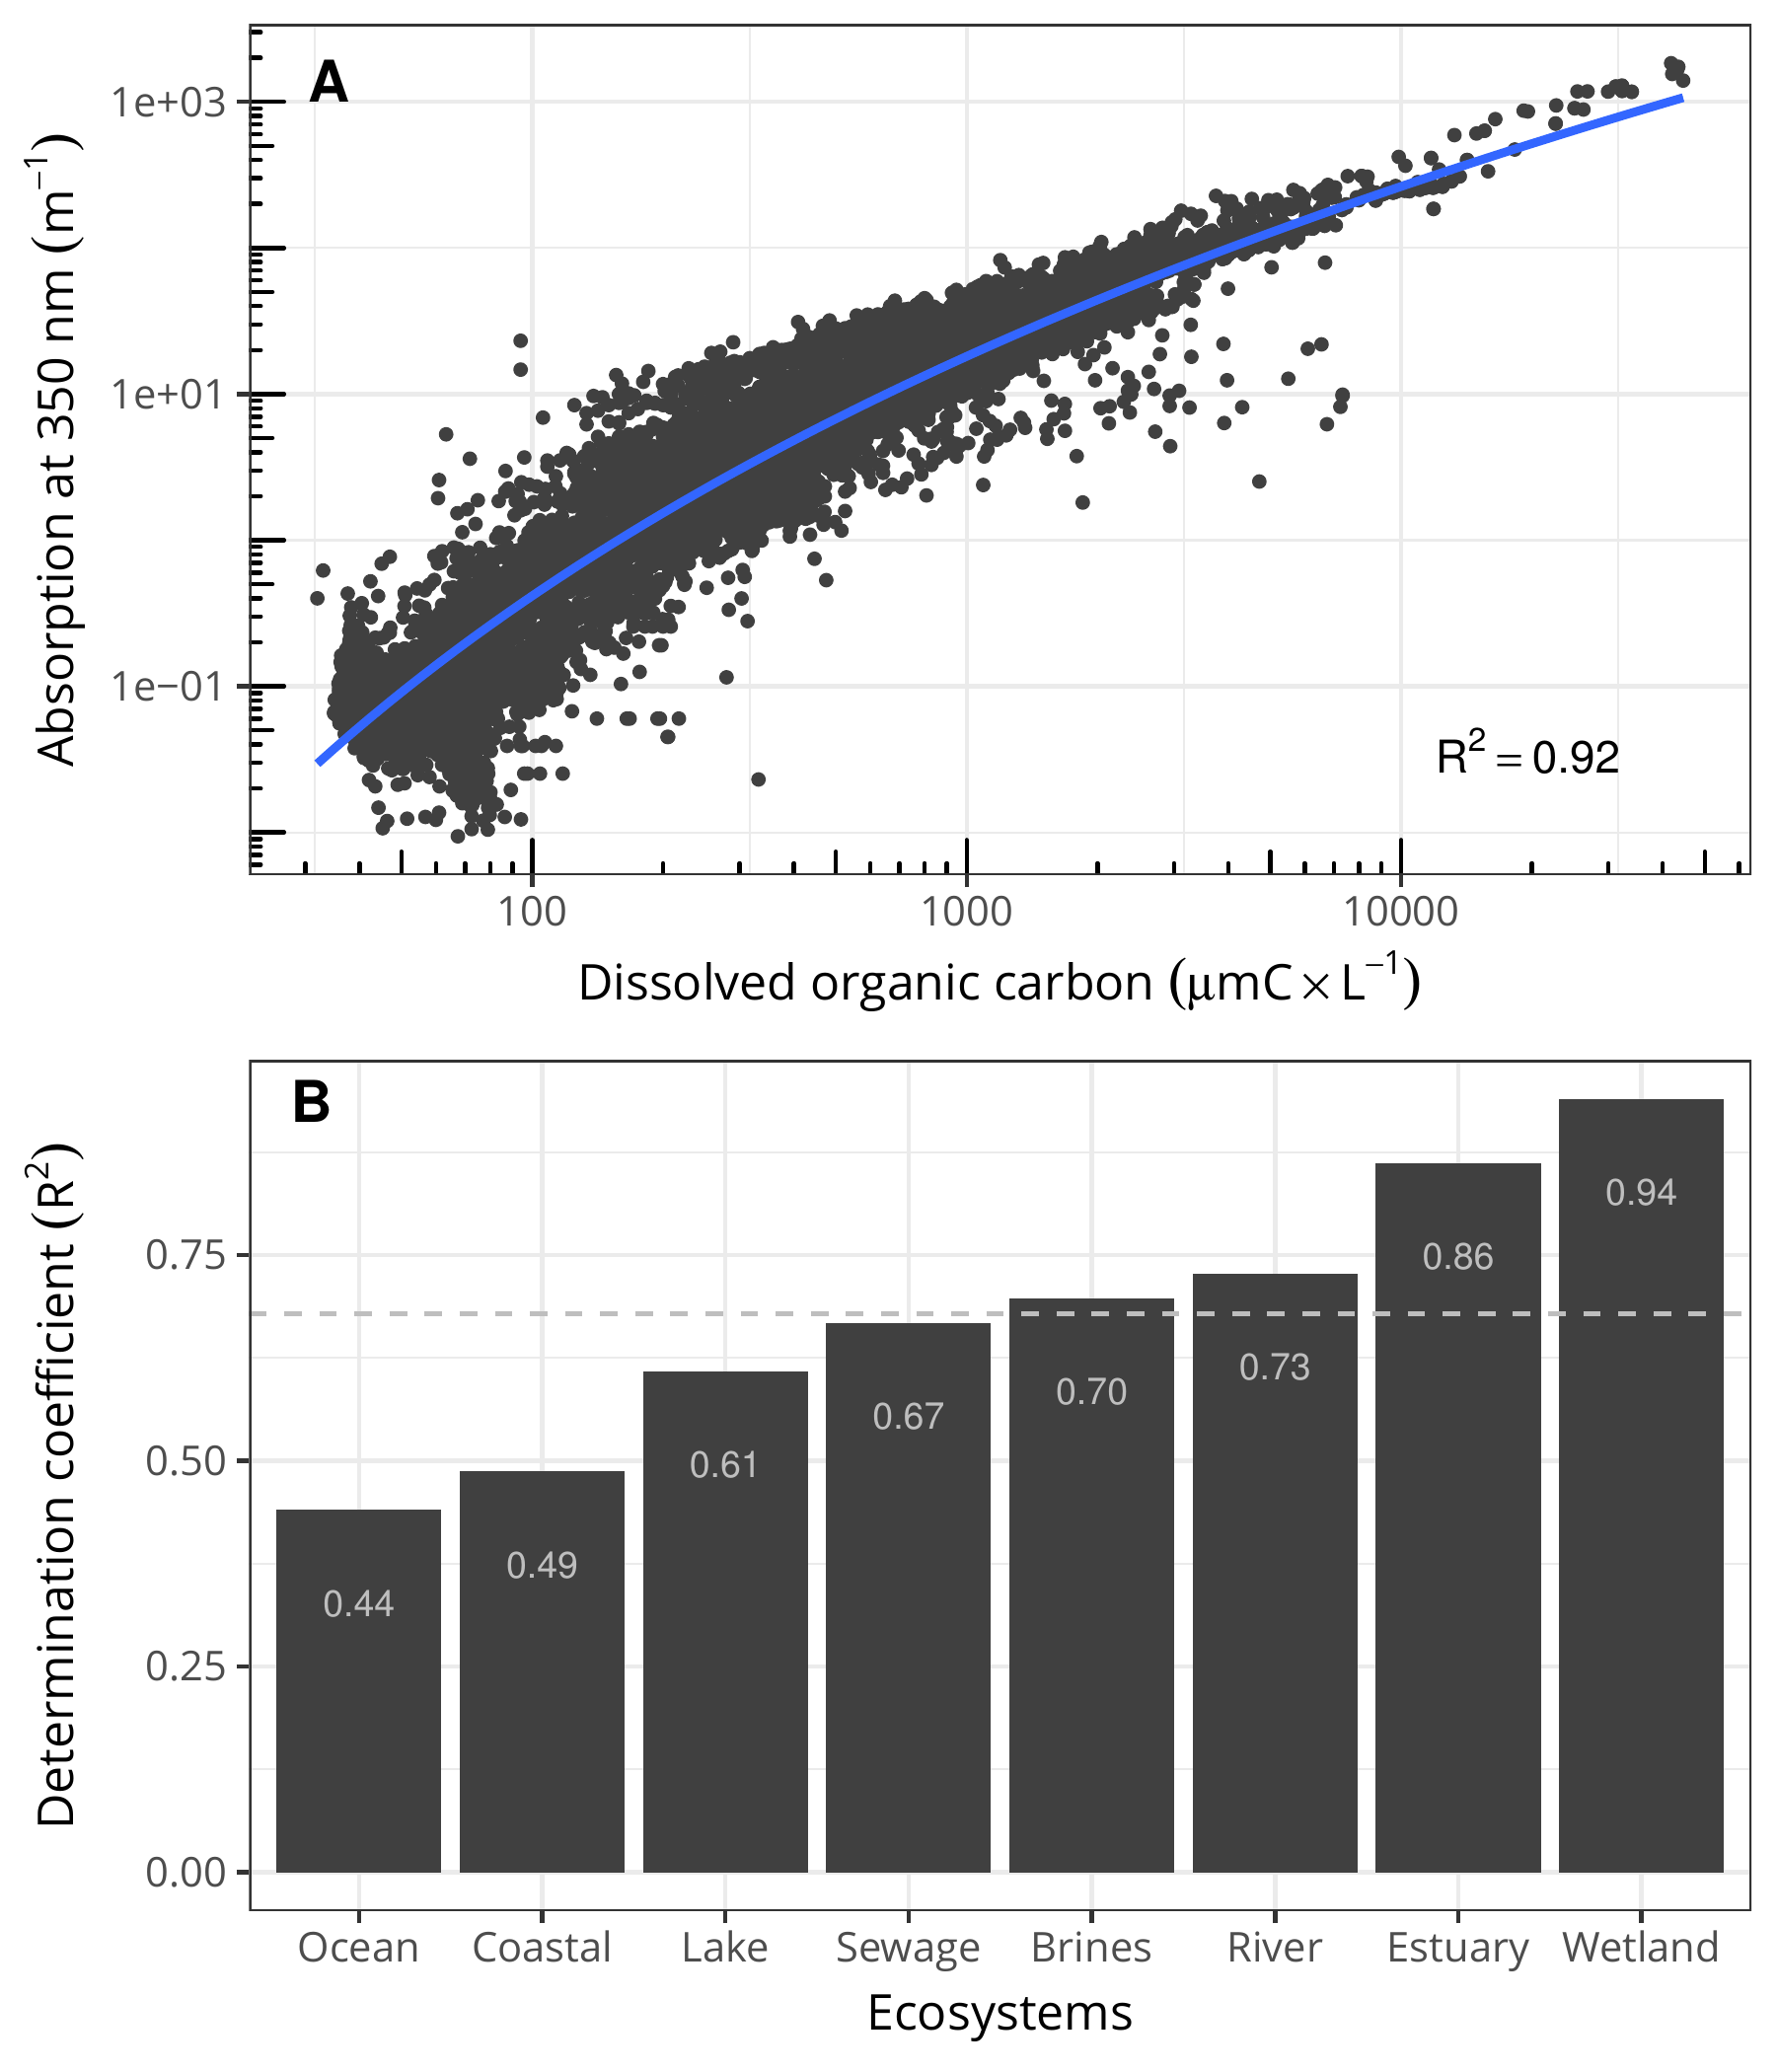
\includegraphics[scale = 1]{../../graphs/fig5}
	\caption{Averaged SUVA\textsubscript{254} calculated using observations from river and ocean ecosystems as a function of the distance to the closest coastline. Positive distances represent inland samples (rivers) whereas negative distances represent oceanic samples. The blue line represents the segmentation analysis performed on the linear relationship between SUVA\textsubscript{254} and distance ($R^2~=~0.95, p~<~0.00001$). Dashed vertical line represents the identified breakpoint at 359 km away from the coastline toward the ocean.}
\end{figure}

\clearpage
\newpage

\begin{figure}[h]
	\centering
	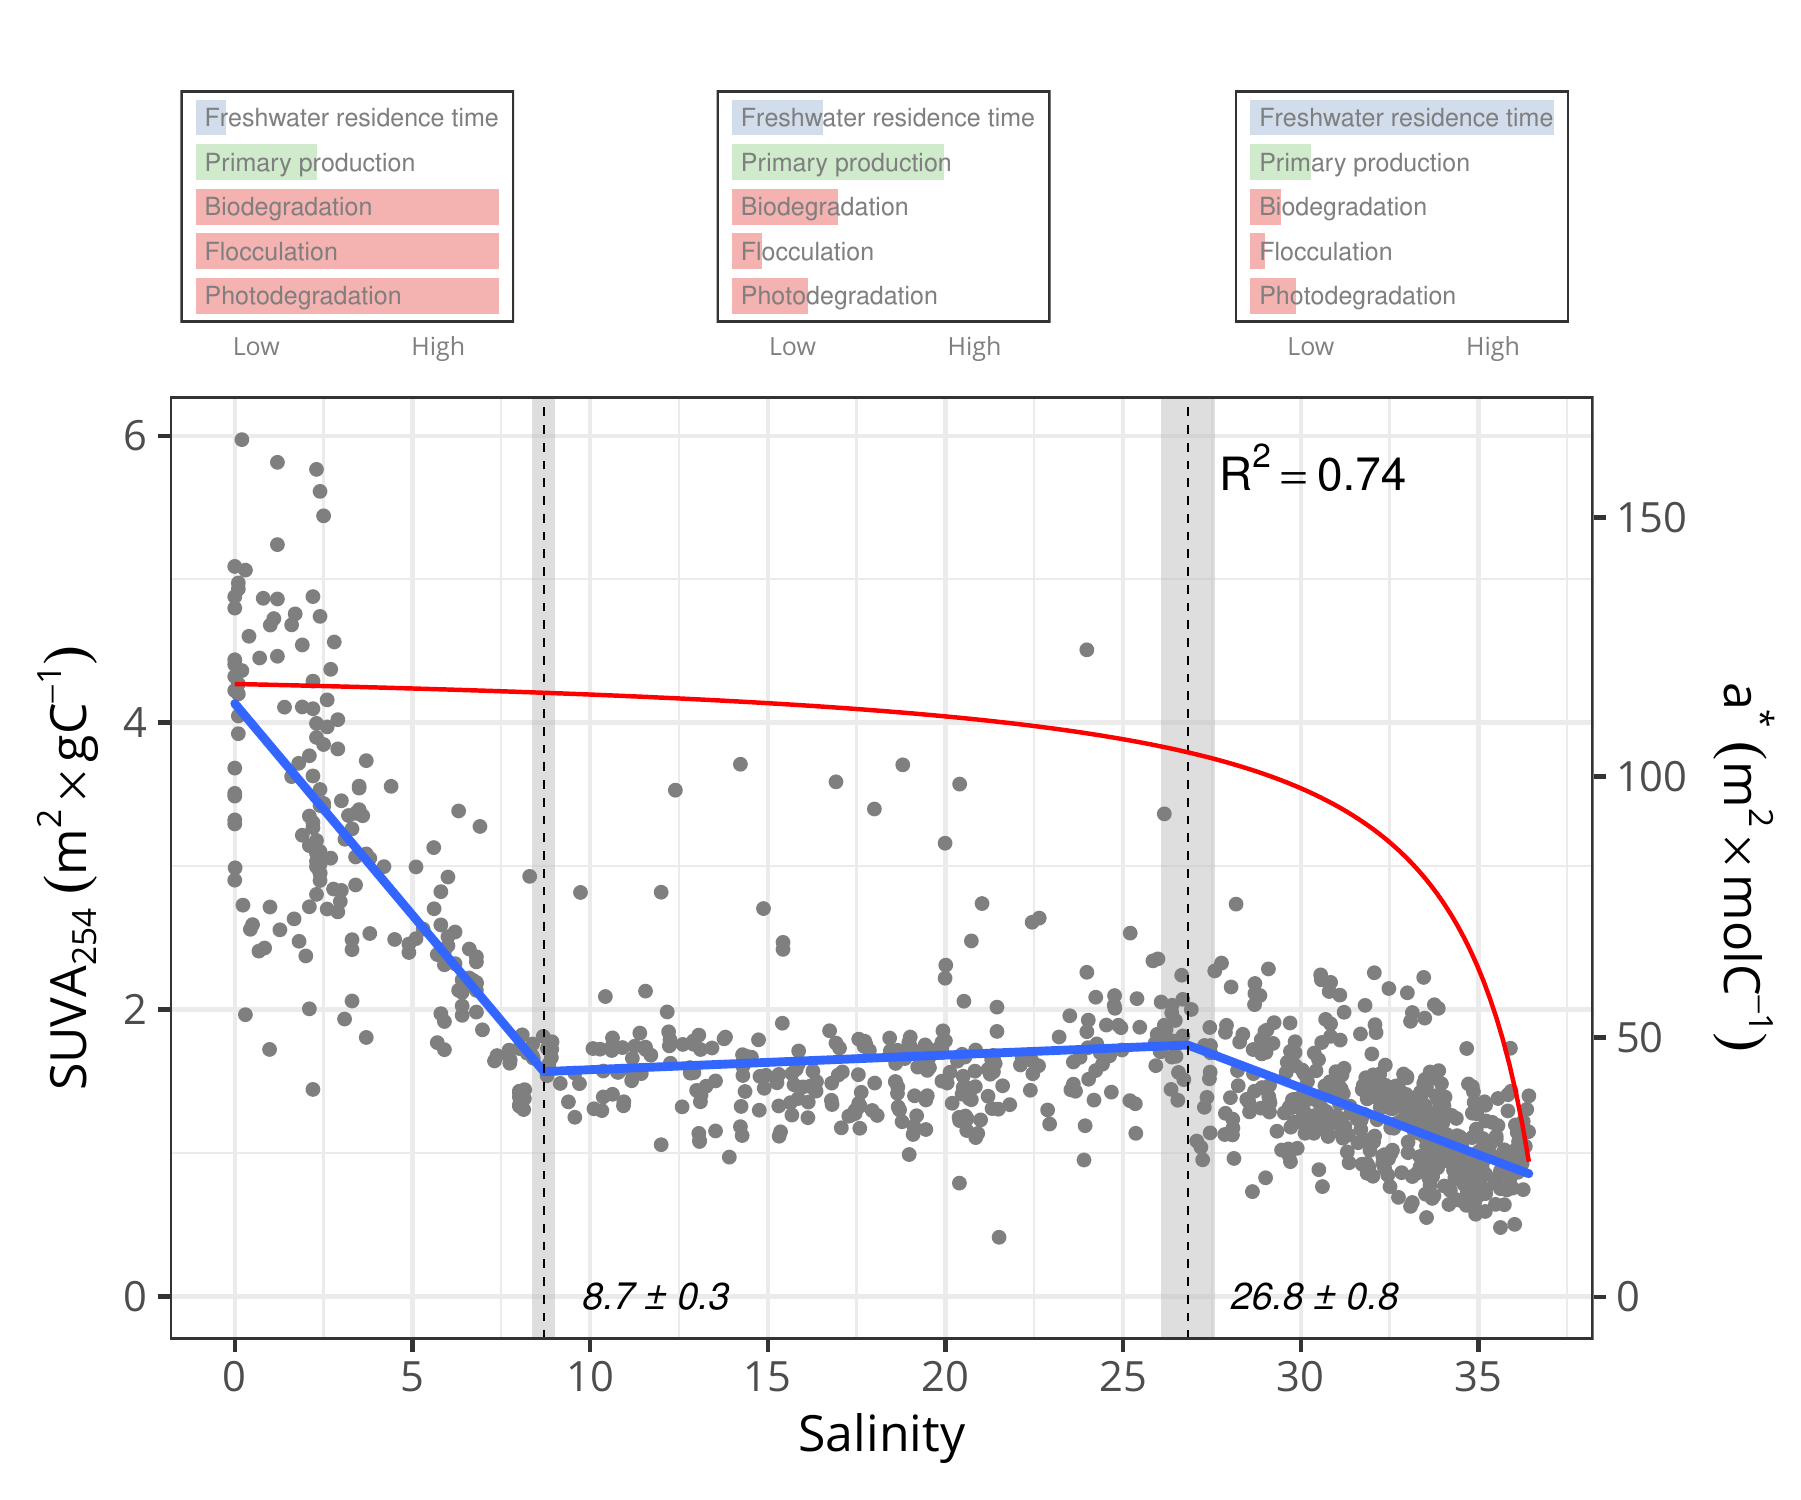
\includegraphics[scale = 1]{../../graphs/fig6}
	\caption{Segmentation analysis performed on the linear relationship between SUVA\textsubscript{254} and salinity ($R^2~=~0.74, p~<~0.00001, n~=~1080$). Dashed vertical lines represent the identified breakpoints at salinity 8.51 and 28.36.}

\end{figure}

\clearpage
\newpage

\begin{figure}[h]
	\centering
	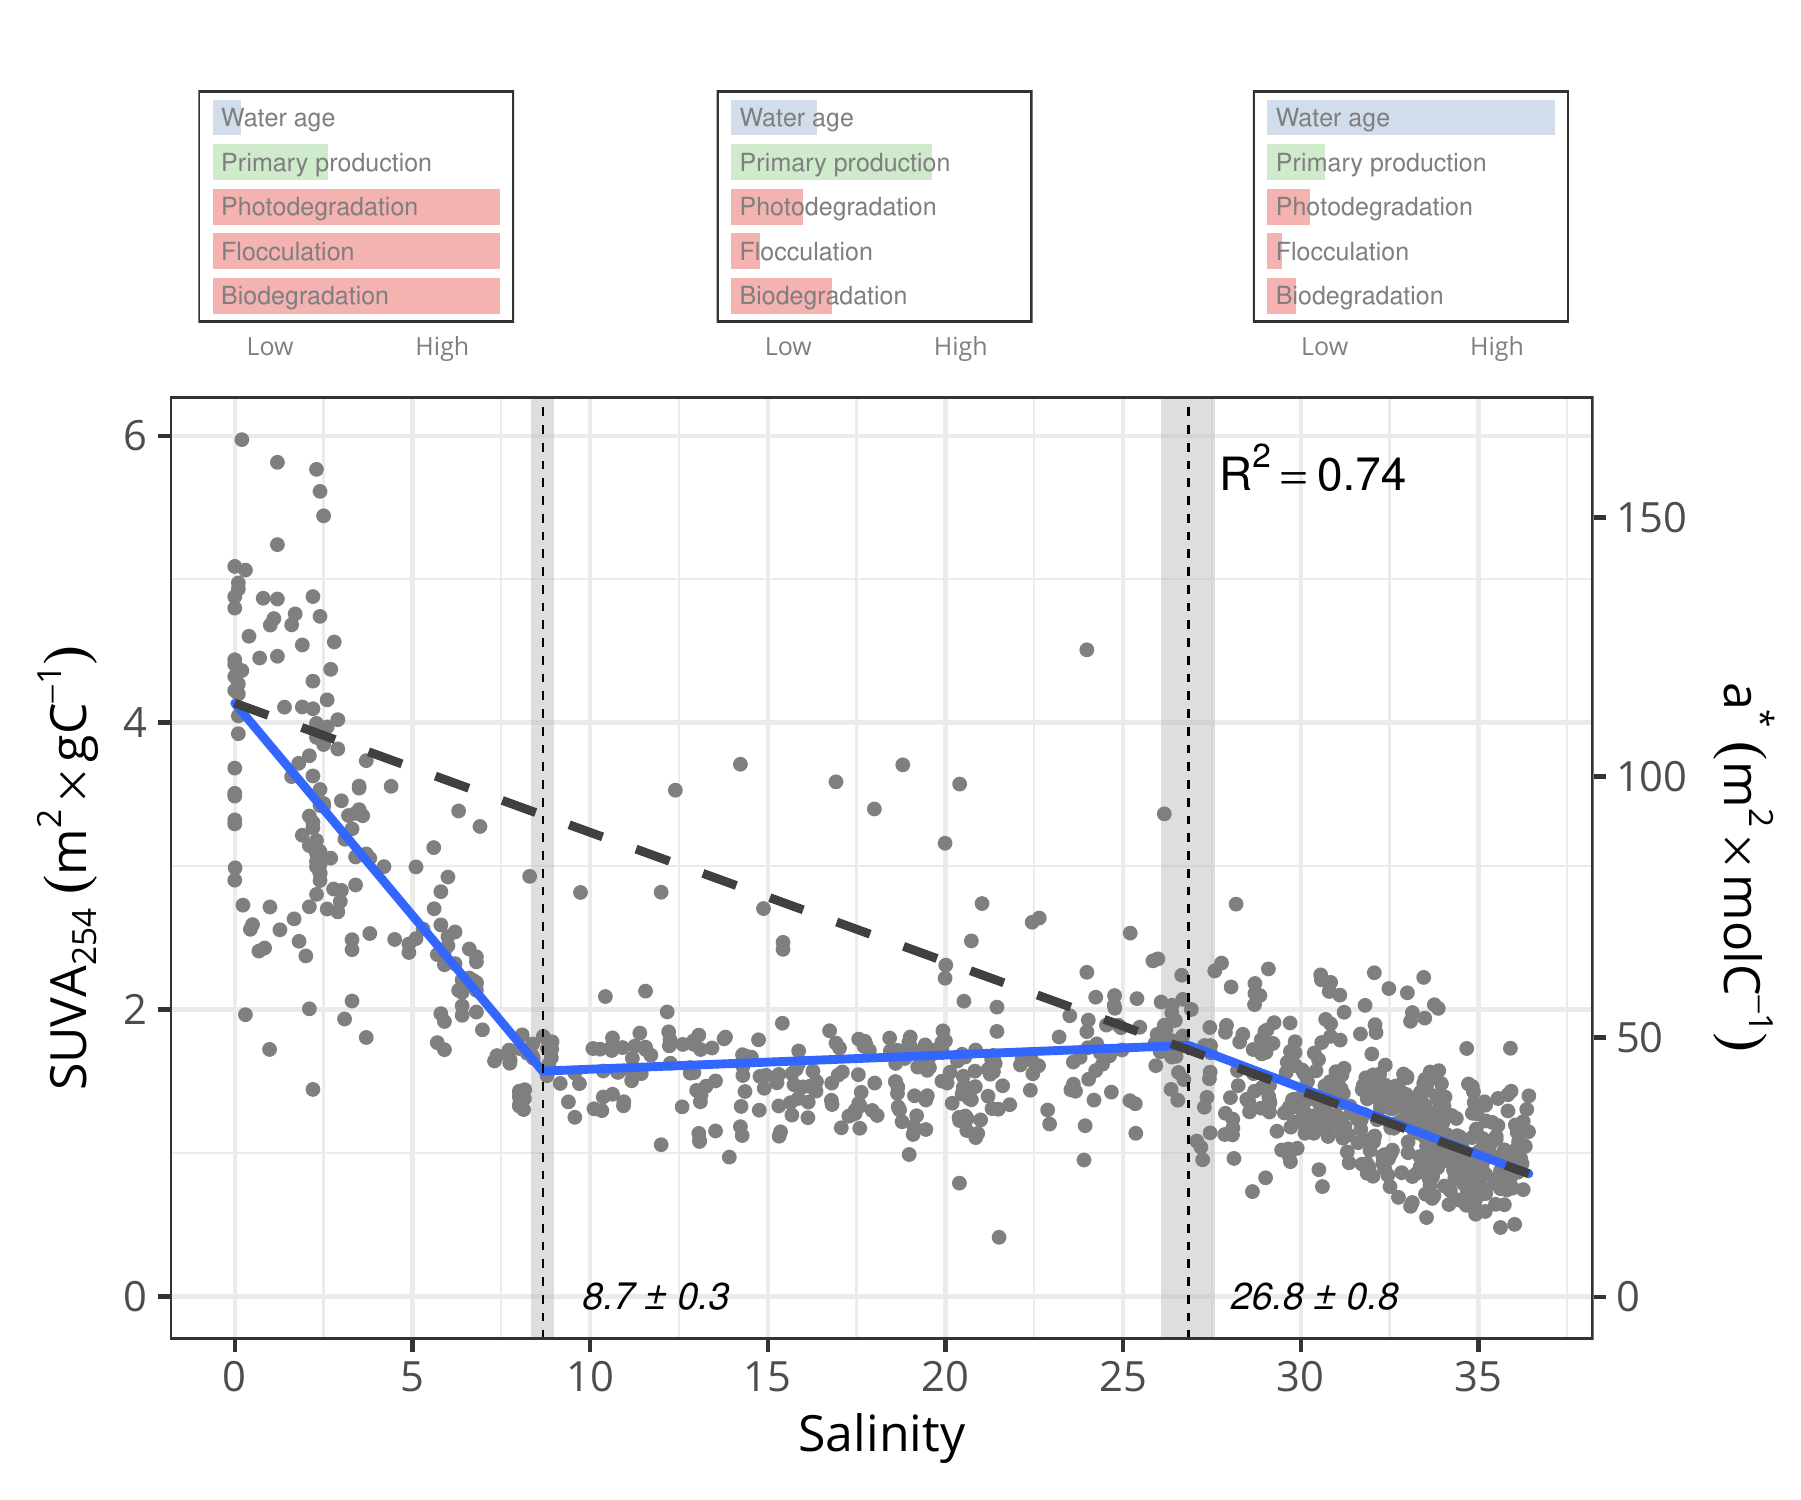
\includegraphics[scale = 1]{../../graphs/fig7}
	\caption{Principal component analysis showing the linear relationships between selected variables ($n = 1841$). The total variance explained by the first two principal components is 67.5\%.}
\end{figure}

\clearpage
\newpage

\begin{figure}[h]
	\centering
	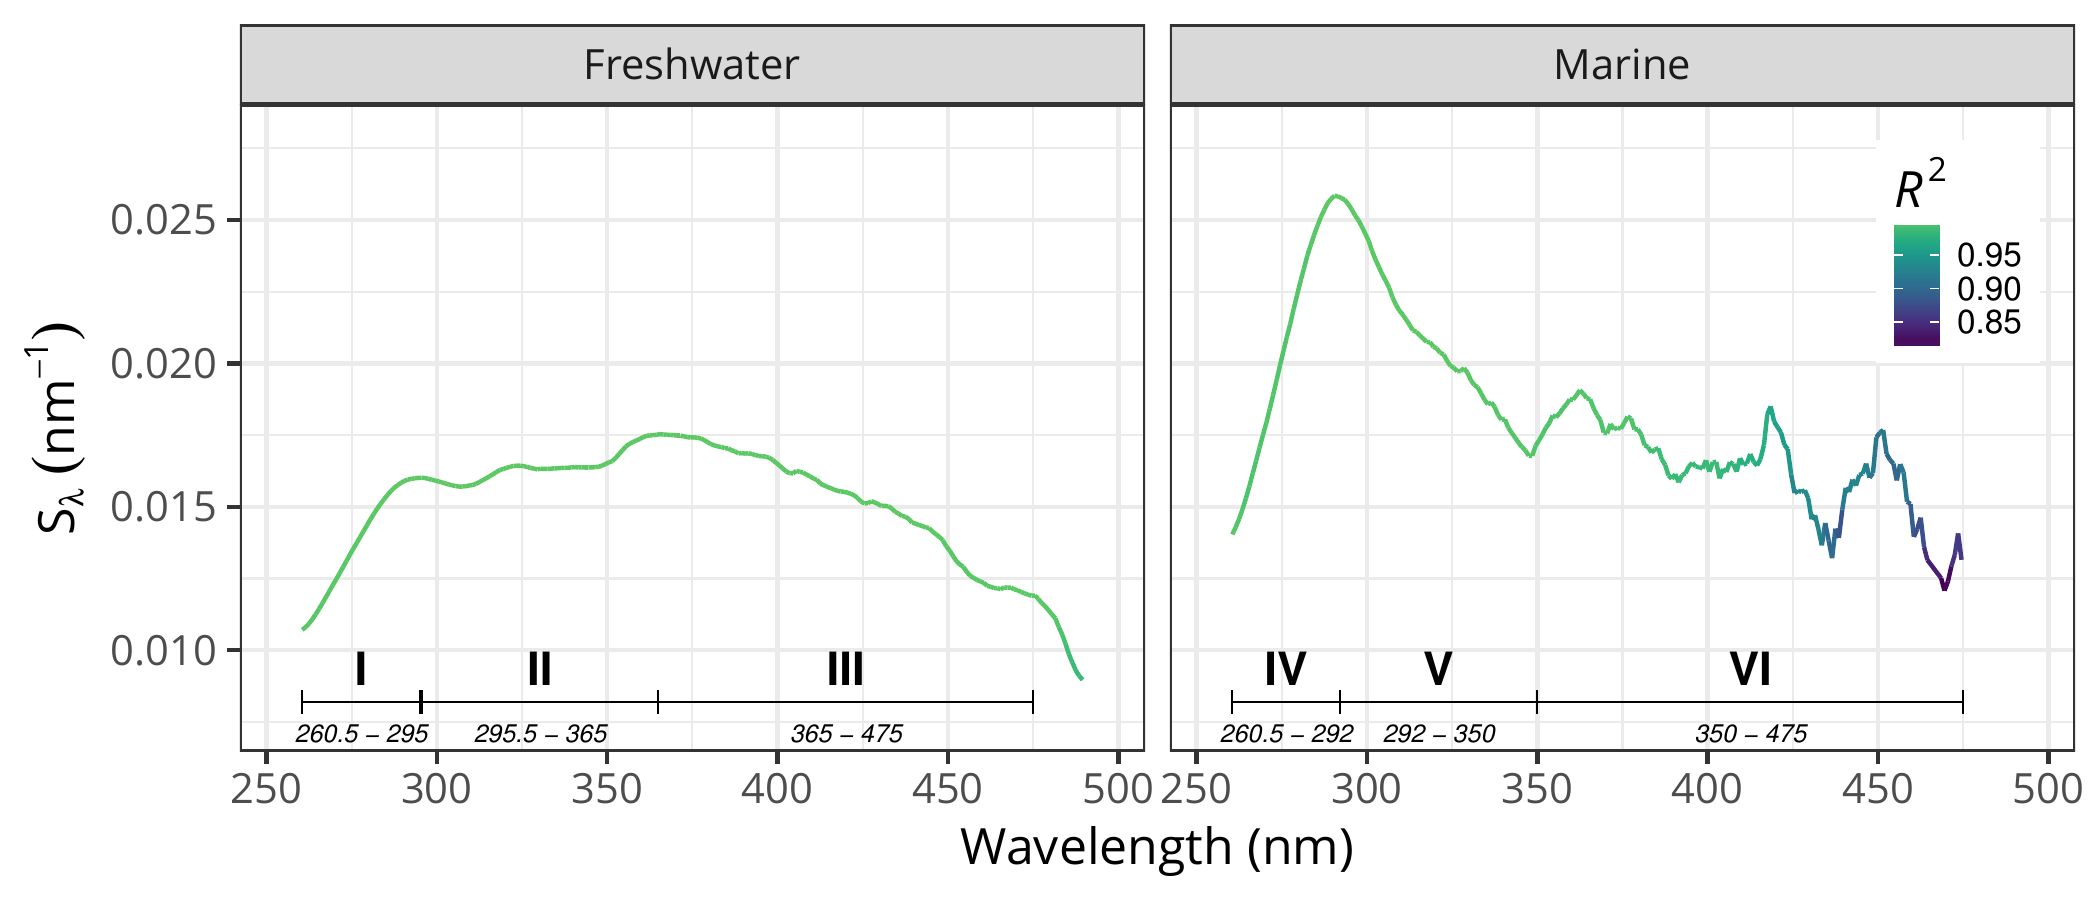
\includegraphics[scale = 1]{../../graphs/fig8}
	\caption{(\textbf{A}) Determination coefficient ($R^2$) showing the goodness of the linear fit between DOC and absorption coefficients measured at different wavelengths for both freshwater and marine ecosystems. (\textbf{B}) Spectral slope curve (S\textsubscript{$\lambda$}) calculated on averaged absorption spectra on freshwater and marine ecosystems using a 21 nm wavelength interval.}
\end{figure}

\end{document}
